\subsection{CU2 Visualizar Menú}
Al momento de ingresar las credenciales y que el sistema otorgue acceso al usuario, aparecerá una pantalla muy simular a la que mostramos a continuación (figura \ref{fig:Pantalla Visualizar Menu - Vista de Escenarios}). Esta pantalla posee el mismo diseño que el inicio de sesión (figura \ref{fig:Pantalla Iniciar Sesion - Vista de Escenarios}), solo que esta vez, se muestran tres opciones principales. 
\begin{itemize}
	\item \textbf{Gestionar Agenda:} En esta opción se desplegará otra pantalla que le dará acceso al usuario a toda la información que desee saber sobre los registros de los vehículos que estén dentro del taller además de la gestión de los mismos.
	\item \textbf{Gestionar Refacciones:} En dado caso que el usuario desee saber sobre la existencia de alguna refacción en particular dentro del almacén del taller además de generar una solicitud para la obtención de una si en necesario.
	\item \textbf{Cancelar:} El usuario desea salir de esa pantalla y regresar a la pantalla de Iniciar Sesión (figura \ref{fig:Pantalla Iniciar Sesion - Vista de Escenarios}).
\end{itemize}
\begin{figure}[!h]
	\centering
	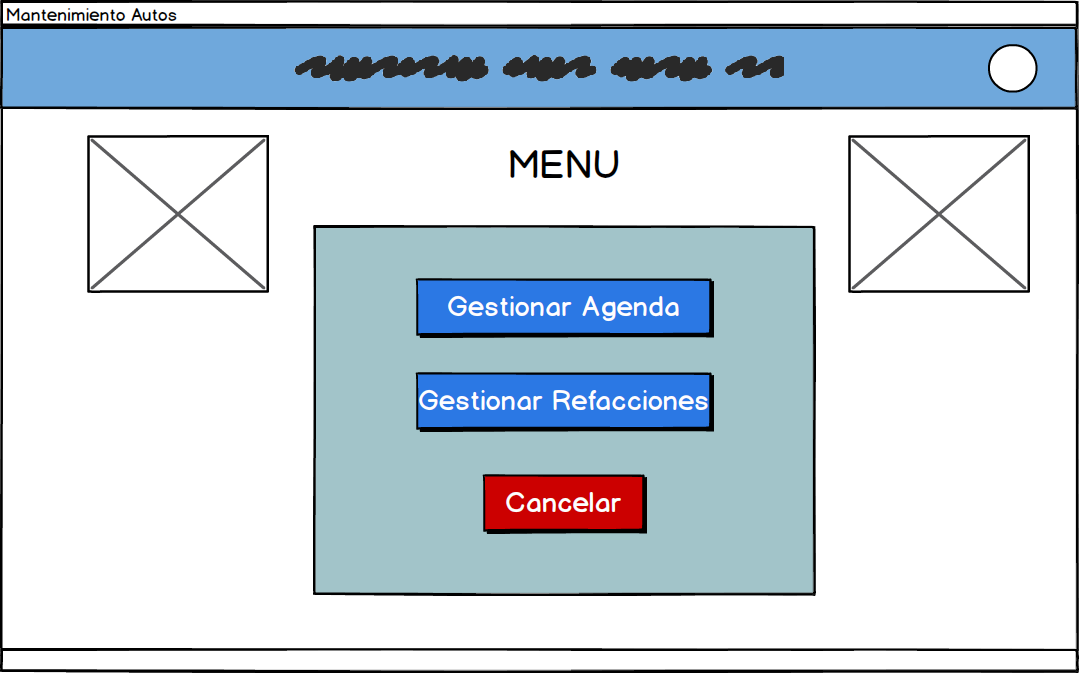
\includegraphics[width=1\textwidth]{./diseno/vescenarios/imagenes/VisualizarMenu}
	\caption{Pantalla Visualizar Menu - Vista de Escenarios}
	\label{fig:Pantalla Visualizar Menu - Vista de Escenarios}
\end{figure}
\clearpage